%-----------------------------------------------------
%  Introduction
%-----------------------------------------------------


\section{서론}
\subsection{연구의 필요성}

천체 관측은 천체 망원경이 대중화됨에 따라 여러 사람들이 시도하는 경우가 많아졌다. 하지만 천체관측을 할 시에는 여러 가지 변수가 존재하여, 천체관측을 어렵게 하는 경우가 있다. 천체 관측을 하는 데 중요한 요소 중 하나는 초점을 정확하게 맞추는 것이다. 초점이 얼마나 정확하게 맞았는 지에 따라서 천체관측한 사진의 상이 얼마나 정확하게 나왔는지가 달라질 뿐만이 아니라 장시간 노출을 하여 사진을 촬영해야 하는 밤에 경우 초점이 맞지 않으면 그 차이가 더욱 두드러지게 나타나게 된다. 최근에는 이러한 문제를 해결하기 위해 컴퓨터를 이용하여 정확한 제어를 통해 짧은 시간안에 효율적인 관측을 진행하고자 노력하고 있다.

\begin{figure}[h]
	\begin{center}
		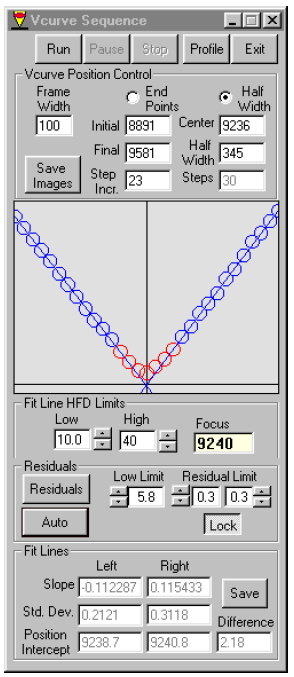
\includegraphics[width = 4cm]{V-curve}
	\end{center}
	\caption{FocusMAX에서 V curve를 얻어 초점을 결정하는 모습 \cite{weber2001fast}.}
	\label{V-curve}
\end{figure}

천체망원경의 초점을 맞추는 대표적인 방법들 중 하나는 천체망원경의 모터포커서를 활용하여 FWHM(Full Width Half Maximum), UFD(Half Flux Diameter)와 같은 값들을 활용한 V-curve를 그리는 방법이다. Fig. \ref{V-curve}이 UFD와 V-curve를 활용하여 초점을 찾은 대표적인 경우로, 이 방법을 활용할 경우 어떤 상황에서도 꽤 정확한 결과를 얻을 수 있지만, 이는 별의 flux 정규분포로 퍼져있어야 정확한 결과를 얻을 수 있다. 만약 퍼져있는 정도가 부정확하면 이 결과를 신뢰성이 낮아지게 되며, 천체 관측시의 온도 및 주변 대기의 상태(seeing)에 많은 영향을 받게 된다. 실제로 Persha(2001)는 주위 온도에 따라서 초점이 변화한다는 점을 보완하고자 이를 보정할 수 있도록 온도 보상 초점 조절 방법을 연구하였다.\cite{persha2001temperature}


본교 보조 관측실은 자동으로 개폐되는 슬라이딩 루프(sliding roof)가 있어, 이곳에 천체망원경을 고정하여 설치해 놓고 관측을 진행하고 있다. 때문에 네트워크만 연결이 되면 언제 어디서든 망원경을 조종할 수 있다는 장점을 가지고 있지만, 아직까지 완전 자동화된 천체관측은 불가능하다. 특히나 V-curve를 사용하는 방법은 경통의 길이를 변화하면서 값을 측정해야하기 때문에 아주 긴 시간이 필요하다는 단점이 있으며, 이는 직접 여러가지 상황을 확인하고 반영하기 어려운 원격 천체관측에 어울리지 않으며, 실제로 학교 주변의 대기 상황이 실시간으로 변하기 때문에 이를 이용하여 정확한 초점을 맞추기는 매우 어렵다.


이런 단점들을 개선하기 위해 마스크를 활용하는 방법이 주목받고 있다. 크게 하트만 마스크와 바흐티노프 마스크의 두 가지로 나뉘는 마스크는 V-curve를 사용하는 것에 비해 관측시에 필요한 시간을 획기적으로 줄일 수 있다는 장점이 있으며, 제작 및 관리에도 용이하기 때문에 천체망원경의 원격 제어에 알맞은 특징들을 지니고 있다.





\subsection{연구 목적}

본 연구에서는 소형 천체망원경의 원격 제어를 위한 효율적인 초점조절방식인 바흐티노프마스크의 제어를 효율적으로 할 수 있도록 하며, 이를 위하여 소형 천체망원경에서 사용할 수 있는 덮개를 제작하여 실제 관측에 적용하는 것을 목적으로 한다. 


제작한 덮개 및 시스템을 위한 펌웨어는 기존에 제작하였던 GS-touch를 개량하여 사용하였으며, GS-touch와 같이 ASCOM(Astronomy Common Object Model)을 지원하여 확장성을 넓힐 수 있도록 계획하였다. GS-touch의 전용 ASCOM driver또한 천체망원경의 원격 제어에 맞추어 개량하여 일반인들 또한 foucsMAX와 같은 천체관측 소프트웨어를 통하여 쉽게 접근할 수 있도록 계획하였다.

\begin{comment}
이를 위해 해결해야 할 주요 문제는 다음과 같다.

\begin{itemize}
	
	\item{덮개는 바흐티노프 마스크를 정확하게 제어할 수 있는가?}\\[-34pt]
	\item{바흐티노프 마스크를 이용하여 초점을 정확하게 맞출 수 있는가?}\\[-34pt]
	\item{향상된 모터포커서를 이용하여 이들을 제어할 수 있는가?}
	
\end{itemize}
\end{comment}

Budding, E.(1995)또한 뉴질랜드 Carter 천체관측소에 자동화된 소형 천체망원경을 설치하여 운영하고 있다. Budding, E.는 소형 천체망원경을 원격제어할 수 있도록 네트워크를 활용하면 일반적인 천체관측에 비해 비용측에서 큰 이득을 보며, 편의성또한 증대할 수 있다고 주장하였다.\cite{budding1995global} 본 연구 또한 소형 천체망원경의 원격 제어를 통해 비용절감 및 편의성 증대 등의 효과들을 얻고자 한다.

\begin{comment}
제작한 모터 포커서 컨트롤러는 GS-touch로 명명하였다. GS-touch는 스테핑 모터를 구동할 수 있고 컴퓨터로 제어할 수 있도록 설계하였으며, 전용 ASCOM (Astronomy Common Object Model) dirver를 개발하여 ASCOM을 지원하는 천문 소프트웨어를 이용하여 쉽게 사용할 수 있도록 하였다.
\end{comment}



\subsection{연구 문제}

본 연구에서 제시하는 연구 문제는 다음과 같다:
\begin{enumerate}
	
	\item 덮개는 바흐티노프 마스크를 정확하게 제어할 수 있는가?
	\item 바흐티노프 마스크를 이용하여 초점을 정확하게 맞출 수 있는가?
	\item 향상된 모터포커서를 이용하여 이들을 제어할 수 있는가?
	
\end{enumerate}
이들을 통해 얻을 수 있는 결과는 다음과 같다.

\begin{enumerate}
	
	\item 일반PC를 통해 천체망원경의 여러 시스템들을 제어할 수 있도록 한다. 이는 카메라의 전원, 가대의 전원 등을 포함하며, 주요 제어대상은 경통의 길이이다.
	\item ASCOM에 따른 표준 초점 제어 시스템을 제공하며, FocusMAX와 같은 천체관측 소프트웨어를 통한 원활한 제어가 가능하게 한다.
	\item 앞서 제시한 모든 시스템을 원격으로 조작할 수 있도록 하며 여러 센서들을 통해 정확하게 제어할 수 있도록 한다.
\end{enumerate}	

R.Godoy(2018)외 5명은 본 실험 결과와 유사한 연구 문제를 제시하였으며\cite{godoy2018control}, 이를 실제로 실험에 활용하였다. 본 결과들을 통해 앞으로 자동망원경을 제작하려는 사람들에게 도움이 되고자 한다.
